When writing program specifications, handling inductive structures is inevitable. In imperative programming languages, this is typically achieved through loops or recursion. In Rocq, there are three primary approaches: (1) built-in higher-order functions or predicates from Rocq's standard library, such as \texttt{length} and \texttt{fold}; (2) user-defined \texttt{Fixpoint} functions, which are custom recursive functions; and (3) user-defined \texttt{Inductive} predicates, which are inductively defined logical relations.

The key distinction between the latter two lies in their executability: \texttt{Fixpoint} definitions are computationally executable within Rocq, whereas \texttt{Inductive} predicates are purely logical relations without computational content. Importantly, these approaches can be freely combined in practice. Consequently, whether a specification is ``executable'' is not a well-defined mathematical concept---a single specification may contain both executable and non-executable components.

% Given this observation, the rigid requirement in \textsc{Clever} that all manual specifications must be non-executable appears overly restrictive. In this work, we focus specifically on \texttt{Fixpoint} usage and provide two versions of our specification suite: one \textbf{permitting} \texttt{Fixpoint} definitions and one \textbf{prohibiting} them. This design enables us to investigate how the availability of \texttt{Fixpoint} constructs influences both specification quality and proof difficulty.

Given this observation, the rigid requirement in \textsc{Clever} that all manual specifications be non-executable appears overly restrictive in a broader specification-generation setting. This constraint is primarily motivated by \textsc{Clever}’s design, where implementations are synthesized directly from specifications within Lean, making executability a potential source of specification leakage and trivial solutions. In contrast, our focus is on evaluating specification quality itself rather than end-to-end code synthesis. Accordingly, we focus specifically on the use of \texttt{Fixpoint} and provide two versions of our specification suite: one \textbf{permitting} \texttt{Fixpoint} definitions and one \textbf{prohibiting} them. This design enables us to systematically investigate how the availability of \texttt{Fixpoint} constructs affects both specification quality and proof difficulty.

% --- 表格 1：LLM 使用情况 ---
\begin{figure}[t]
    \centering
    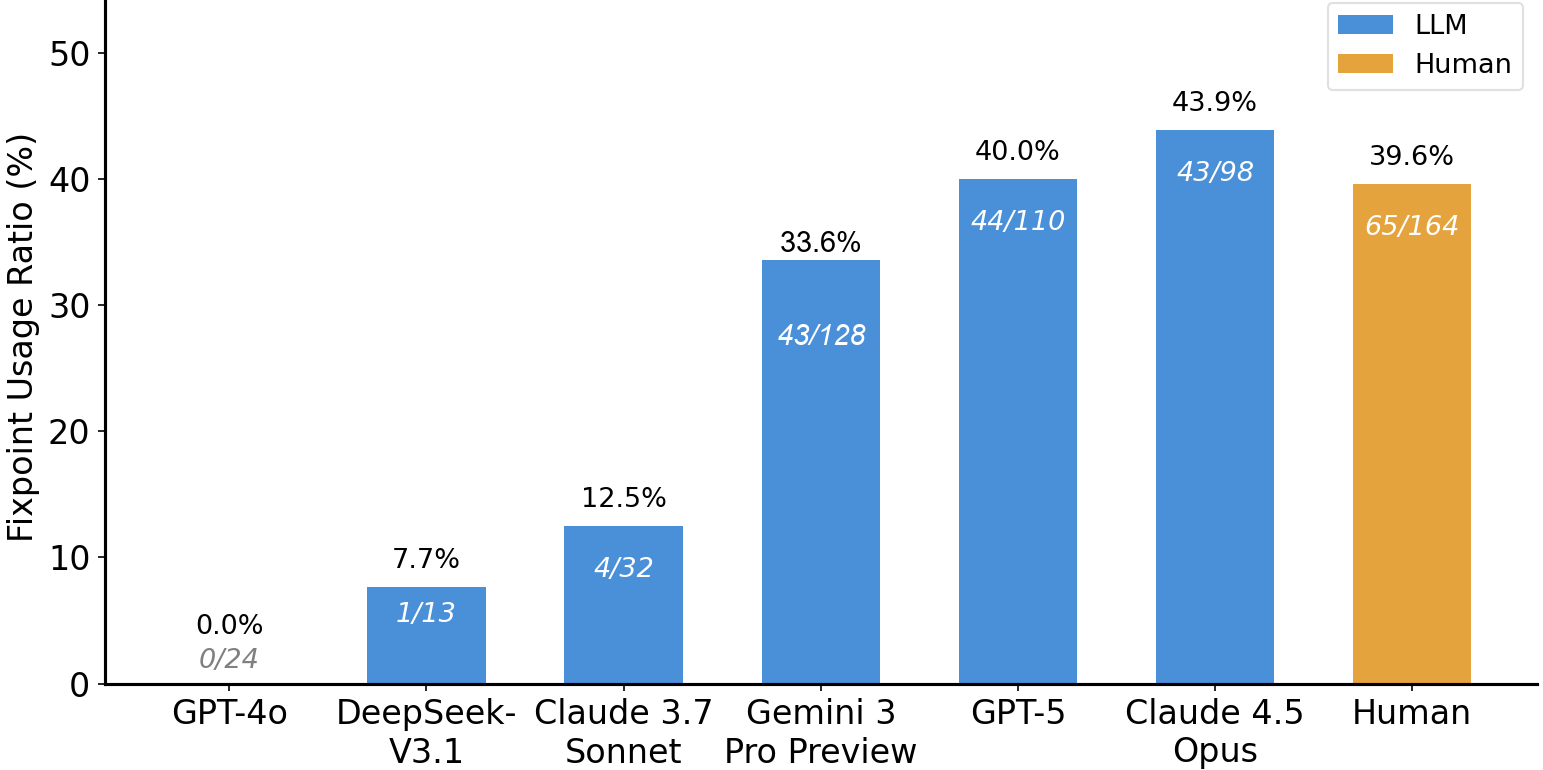
\includegraphics[width=0.9\linewidth]{images/fixpoint_usage.png}
    \caption{Frequency of \texttt{Fixpoint} usage across specifications. The three strongest LLMs exhibit usage ratios (33.6--43.9\%) comparable to human (39.6\%).}
    \label{fig:fixpoint-usage}
\end{figure}


Figure~\ref{fig:fixpoint-usage} presents the frequency of \texttt{Fixpoint} usage in specifications. A clear divide emerges: weaker models (GPT-4o, DeepSeek-V3.1, Claude 3.7 Sonnet) rarely employ \texttt{Fixpoint} constructs, while stronger models (Gemini 3 Pro Preview, GPT-5, Claude 4.5 Opus) utilize them substantially more often (33.6--43.9\%). Notably, human experts exhibit a similar ratio of approximately 40\%, suggesting that state-of-the-art models have developed comparable judgment in determining when recursive structures are necessary for precise formalization.

\begin{figure}[t]
    \centering
    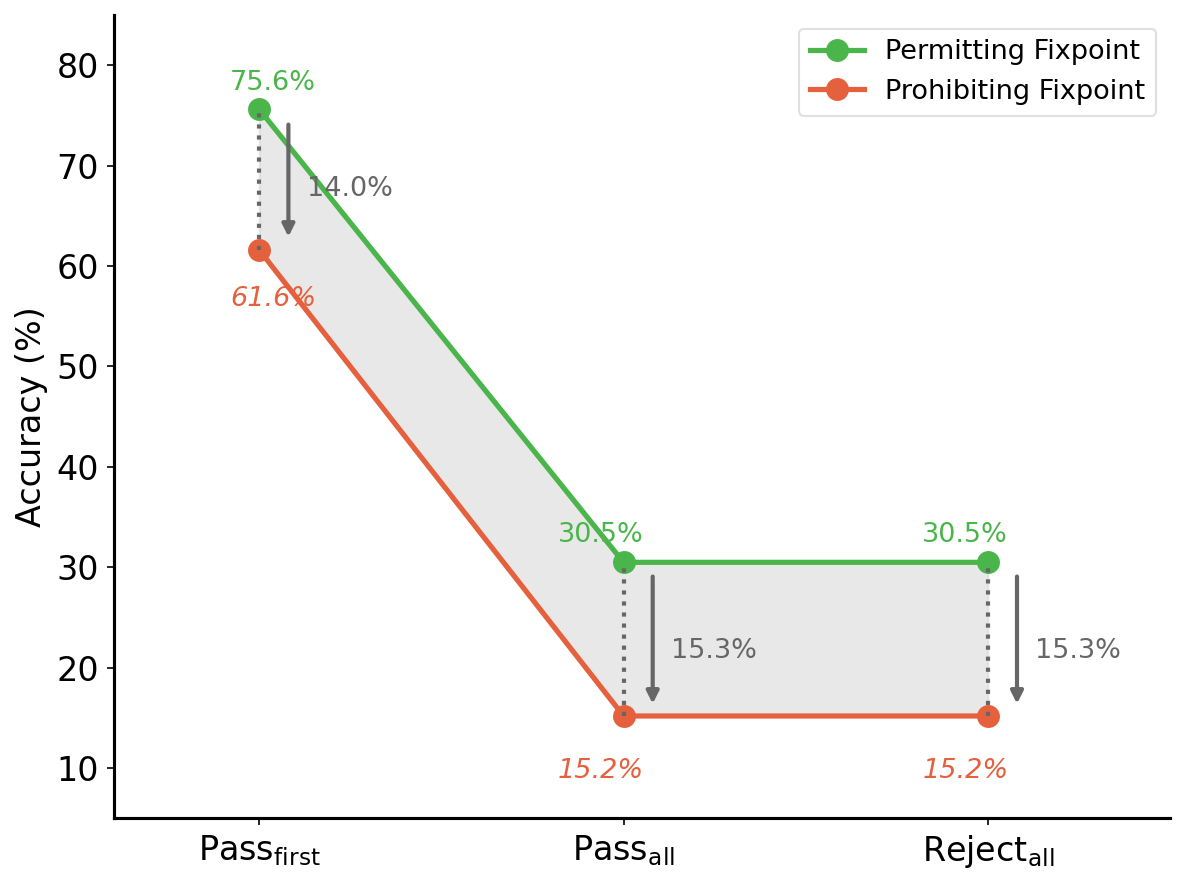
\includegraphics[width=0.82\linewidth]{images/fixpoint_impact.png}
    \caption{Impact of prohibiting \texttt{Fixpoint} on human specification quality ($n=164$). Disallowing recursive constructs leads to substantial performance drops across all metrics.}
    \label{fig:fixpoint-impact}
\end{figure}

This pattern indicates that \texttt{Fixpoint} plays a crucial role in effective specification design. To validate this hypothesis, we evaluated Gemini 3 Pro Preview on both versions of our human-written specifications. As shown in Figure~\ref{fig:fixpoint-impact}, proofs against specifications prohibiting \texttt{Fixpoint} are substantially harder, with a notable drop in the success rate. Furthermore, specifications without \texttt{Fixpoint} require significantly more lines of code and exhibit lower readability, as complex recursive logic must be manually unfolded into verbose relational rules. These results lead to the following finding:


\begin{tcolorbox}[
  colback=gray!10,
  colframe=gray!60,
  boxrule=0.6pt,
  arc=2pt,
  left=6pt,
  right=6pt,
  top=6pt,
  bottom=6pt
]
\small
\label{executable}
\textbf{Executable Components Matter.} Well-designed specifications benefit significantly from executable components. Encapsulating sub-logic within \texttt{Fixpoint} definitions effectively reduces both specification complexity and verification difficulty. Pure relational specifications, while theoretically elegant, lead to verbose code and unwieldy proof obligations that challenge even the strongest models.
\end{tcolorbox}
